\documentclass{beamer}
%
% Choose how your presentation looks.
%
% For more themes, color themes and font themes, see:
% http://deic.uab.es/~iblanes/beamer_gallery/index_by_theme.html
%
\mode<presentation>
{
  \usetheme{Madrid}      % or try Darmstadt, Madrid, Warsaw, ...
  \usecolortheme{crane} % or try albatross, beaver, crane, ...
  \usefonttheme{default}  % or try serif, structurebold, ...
  \setbeamertemplate{navigation symbols}{}
  \setbeamertemplate{caption}[numbered]
  
} 

\usepackage[english]{babel}
\usepackage[utf8x]{inputenc}
\usepackage{courier}
\usepackage{dsfont}
\usepackage{verbatim} 
\usepackage{tikz}
\usepackage{caption}
\usepackage{multirow}
\usepackage{venndiagram}
\usepackage{xcolor}
\usepackage{enumitem}
\usepackage{listings}
\usepackage{hyperref}
\hypersetup{
    colorlinks=true,
    linkcolor=blue,
    filecolor=magenta,      
    urlcolor=cyan,
}

\newcommand{\code}[1]{\texttt{#1}}

\usetikzlibrary{shapes,decorations,arrows,calc,arrows.meta,fit,positioning}
\tikzset{
    -Latex,auto,node distance =1 cm and 1 cm,semithick,
    state/.style ={ellipse, draw, minimum width = 0.7 cm},
    point/.style = {circle, draw, inner sep=0.04cm,fill,node contents={}},
    bidirected/.style={Latex-Latex,dashed},
    el/.style = {inner sep=2pt, align=left, sloped}
}



\setitemize{label=\usebeamerfont*{itemize item}%
  \usebeamercolor[fg]{itemize item}
  \usebeamertemplate{itemize item}}

\newcommand{\Mypm}{\mathbin{\tikz [x=1.4ex,y=1.4ex,line width=.1ex] \draw (0.0,0) -- (1.0,0) (0.5,0.08) -- (0.5,0.92) (0.0,0.5) -- (1.0,0.5);}}%

\title[UIowa Biostatistics]{Prospectus title}
\subtitle{and subtitle!}
\author{Collin Nolte}
\date{April 22, 2022}

\begin{document}

\begin{frame}
  \titlepage
\end{frame}

\begin{frame}{Outline}
  \tableofcontents
\end{frame}

\section{Problem statement}
\section{Existing results}
    \subsection{Method 1}
    \subsection{Method 2}
    \subsection{Method 3}
\section{Comparative study}
\section*{References}

\begin{frame}{Problem statement}

\end{frame}

\begin{frame}{Overview}
\begin{center}
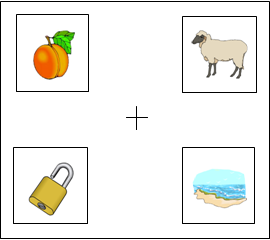
\includegraphics[scale=0.4]{img/visual_world_display.png}
\end{center}
\end{frame}



\begin{frame}{overview 2}
The current method employed by \code{bdots} is to fit the observed $y_{it}$ to an underlying curve $f_{\theta}$, the fitting step given by 
  \begin{align*}
  F: \{y\} \times f \rightarrow N \left(\hat{\theta}_i, \hat{\Sigma}_{\theta_i} \right)
  \end{align*}

Such that
  \begin{align*}
  \hat{\theta}_i = \text{argmin}_{\theta} \  ||y_{it} - f_{\theta}(t)||^2
  \end{align*}

These could be further specified by indicating a group for the observation $g = 1, \dots, G$, where an individual may be in multiple groups (and ultimately, it will be group values being compared)
\end{frame}

\begin{frame}{bdots}
Bootstrapped difference in time series, paper originally by olseon, ecavanaugh, mcmurray, and brown \newline

package written by seedorff \newline

blah blah blah
\end{frame}

\begin{frame}{bdots2}
Current implementation of \code{bdots} involves three steps:
\begin{enumerate}
\item[1.] \textbf{Curve Fitting:} Fitting parametric curve to observed data
\item[2.] \textbf{Curve Refitting:} Manually estimating parameters in case of poor fit
\item[3.] \textbf{Bootstrap} Bootstrap curves to estimate group population curve \newline
\end{enumerate}
I also added a whole bunch of shit to make this package better
\end{frame}

\begin{frame}{bdots add stuff}
One function, \code{bdotsFit}, which can fit any curve to data (previously, one function for each curve) \newline 

Allows for arbitrary user-defined function to be used \newline 

Object returned by bdotsFit very flexible, allows formula definition of bootstrapping difference in bootstrap step \newline 

ggplot, correlation with fixed vector, just general all around better

Refitting step is interactive, can upload external data, saves progress \newline 

\end{frame}

\begin{frame}{compare}
maybe show old bdots vs new bdots, if i can find working code
\end{frame}

\begin{frame}{bdots fit process}
really, this covered in overview 2 slide
\end{frame}

\begin{frame}{bdots bootstrap process}
Here, we perform $B$ bootstraps of the subject parameters to construct bootstrapped curves and confidence intervals. Assuming that each subject is in one \textit{group}, we draw $B$ samples of $\hat{\theta}_i$, where 
\begin{align*}
\hat{\theta}_{ib} \sim N \left(\hat{\theta_i},  \Sigma_{\hat{\theta}_i} \right)
\end{align*}
resulting in a $B\times p$ matrix, denoted $M_i$. \newline 

Doing this for each subject, we construct a $B\times p$ matrix of the average of bootstraps across iterations, 
\begin{align*}
\overline{M} = \frac1n \sum_{i}^n M_i
\end{align*}
(potentially confusing here -- each subject has their own set of parameters, as distinct from group level pars?)
\end{frame}

\begin{frame}{bootstrap cont}
$\overline{M}$ is again a $B \times p$ matrix, each row  representing the average parameter estimate of $\theta$ at each bootstrap $b$. \newline 

Each $1\times p$ row of $\overline{M}$ returns a $1 \times T$ vector representing estimations of $f_{\theta}$ at each point $t$. Together, we have the $B \times T$ matrix $\overline{M}_f$. This gives an estimated fixation curve, 
\begin{align*}
\hat{f} = \frac1B \sum_{b=1}^B \overline{M}_{\{b, \cdot\}_f}, \qquad \widehat{\text{se}}_{f} = \left[ \frac{1}{B-1} \sum_{b=1}^B \left( \overline{M}_{\{i, \cdot\}_{f}} - \hat{f} \right)^2 \right]^{1/2} 
\end{align*}
\end{frame}

\begin{frame}{bdots need}
Have to tighten up functions \newline 

possibly jacknife \newline 

Look at replacing gnls with something else \newline 

still focus on not making vwp specific
\end{frame}

\begin{frame}{Eyetracking data}
In the context of vwp, subjects are lead through trials, with headsets monitoring eye position every 4ms. \newline \\

Two types of events make up eyetracking data: \textit{saccades} and \textit{fixations} \newline \\

A \textit{saccade} represents the physical movement of an eye, lasting between 20-200ms. There is also about a 200ms oculomotor delay between planning an eye movement and it occuring \newline \\

A \textit{fixation} is characterized by a lack of movement, in which the eye is fixated on a particular location. The length of a fixation is more  variable \newline \\

Together, a saccade, followed by a subsequent fixation, is known as a \textit{look}
\end{frame}

\begin{frame}{Fixation curve}
We define a \textit{fixation curve}, $f_{\theta}(t)$ or $f(t  | \theta)$ to represent a (usually parametric) function indicating the probability of fixating on a target at some time, $t$. \newline \\
To disambiguate the term ``target" when used in the VWP, we will let ``Target" denote the object corresponding to a spoken word, while ``target" will denote an object of interest \newline \\

For example, with the four-parameter logistic, our target is typically the Target, while for the six-parameter double-gauss, our target is the Cohort
\end{frame}

\begin{frame}{VWP and looks}
Need for a grounding hypothesis linking eye tracking to cognitive activity \newline \\

Magnuson paper on this, also assumptions from Bob's princess bride \newline \\

For this dissertation, we will ignore the cognitive process and instead focus on recovering underlying fixation curves from observed data. The link between these two can be somebody elses' dissertation. \newline \\

What we will consider here in review is high frequency sampling (HFS) and fixation-based sampling, augmented for target (FBS+T)

\end{frame}

\begin{frame}{Sampling Paradigms}
Two main assumptions focusing on right now: HFS and FBS+T (bob's paper) \newline

\textbf{HFS:} High frequency sampling assumption, "if researcher is sampling at 4ms intervals, the fixation curve is assumped to derive from a probabilistic sample every 4ms" \newline 

\textbf{FBS+T:} Fixation-based sampling + target, series of discrete fixations with reasonable refractory period, treats fixations as primarily a readout ouf the unfolding decision, ignores the role of the fixation as an information gather behavior (pg 26 of princess bride), allows fixations to target to be slightly longer (once fixated, subject more likely to stay)
\end{frame}

\begin{frame}{Importance of sampling paradigms}
Why do we care? Well, it's relevant to the reconstruction of the curve. Specifically, either of these assumptions can be used to simulate eyetracking data. With recovery of the underlying fixation curve being our goal, we should be able to recover the underlying curve according to a particular hypothesis \newline 

To be covered later, but ideally we have a simulation the empirically matches data collected from eyetracking. While we don't quite have that yet, we have two we can explore
\end{frame}

\begin{frame}{High Frequency Sampling}

For subjects $i = 1, \dots, n$, trials $j = 1, \dots, J$, and time points $t = 1, \dots, T$, the current method of estimating this curve is 

\begin{align*}
y_{it} = \frac{1}{J} \sum_{j=1}^J z_{ijt}
\end{align*}
where $z_{ijt} = \{0,1\}$, conditional on the measured fixation at timepoint $t$ in trial $j$. \newline \\
Everything above this is independent of HFS and should go on slide comparing saccades to proportion fixations \newline \\

Under the HFS assumption (employed by bdots), the vector $y_i$ serves as a direct observation of $f_{\theta}(t)$ for subject $i$ ($f_{\theta_i}(t)$?)
\end{frame}

\begin{frame}{HFS wrong}
its wrong. bob even said so \newline \\

but look, plots are fine
\end{frame}

\begin{frame}{FBS+T}
\begin{enumerate}
  \item[1] fixations follow gamma distribution
  \item[2] extra time for target
  \item[3] doesn't take into account prior information (no learning)
\end{enumerate}
\vspace{5mm}
there are also some plots showing bias
\end{frame}

\begin{frame}{Mathematical Structure of Problem}
The primary variable of interest is the \textit{underlying activation curve}, $x \equiv x(t)$, a cognitive process neither measured or observed \newline

Some function of this process is captured by a \textit{fixation curve}, $H(x) = y$(?), which, depending on the context (target or competitor), is represented by a parametric function $f(t|\theta)$ or $f_{\theta}(t)$ \newline 

For subjects $i = 1, \dots, n$, trials $j = 1, \dots, J$, and time points $t = 1, \dots, T$, the current method of estimating this curve is 

\begin{align*}
y_{it} = \frac{1}{J} \sum_{j=1}^J z_{ijt}
\end{align*}
where $z_{ijt} = \{0,1\}$, conditional on the measured fixation at timepoint $t$ in trial $j$.
\end{frame}



\begin{frame}{Fixation vs Sacade}
Current methods employ
\begin{align*}
y_{it} = \frac1J \sum_{j=1}^J z_{ijt}
\end{align*}
where $z_{ijt}$ denotes the \textit{fixation} of subject $i$ in trial $j$ at time $t$. Insomuch as $y_{it}$ represents the observed $f_{\theta}(t)$, we have an issue in that $f_{\theta}(t)$ represents the probability of \textit{fixating} on a target at time $t$, rather than the proportion of fixations already on the target at $t$ \newline \\

In other words, we looking at the wrong thing
\end{frame}

\begin{frame}{fix vs saccade sim}
just use fbs+t paradigm, really, since other one is wrong (and not biased)
\end{frame}

\begin{frame}{identity theroem and time windows}
The identity theorem for analytic functions states: given functions $f$ and $g$ analytic on (open and connected) domain $D$, if $f = g$ on some $S \subseteq D$, where $S$ has an accumulation point, then $f = g$ on $D$ (wikipedia) \newline \\

In other words, letting $D$ be time, if we were able to identify values $\hat{\theta}$ such that $f_{\hat{\theta}} = f_{\theta}$  some interval $S$, then we should find that $f_{\hat{\theta}} = f_{\theta}$ on $D$ \newline \\

In other words again, if we could identify some interval where our approximation of $f$ was best, we could extrapolate this for the rest of the domain
\end{frame}

\begin{frame}{id theorem + window}
In most contexts, we have $f_{\theta}(t) \sim Bern(p(t))$ where $var(p(t)) = p(t) (1-p(t))$, the least amount of variability will occur as $p(t)$ approaches $0$ or $1$ \newline \\

Taking the logistic curve as an example, this will be towards the beginnings and ends of a trial, with maximal variability occuring at the crossover points
\end{frame}

\begin{frame}{window sims}
Here, we run simulations assuming fbst and reconstruct fits using bdots \newline \\

Plot them as-is, along with 200ms shift to account for occulomotor delay \newline \\

To examine various time windows, have included simulations that will sample at a fixed rate (every 25ms) within a specified time interval, rather than relying on length of fixations or identified target \newline \\

Each simulation is based off a singular underlying fixation function with identical parameters across trials
\end{frame}

\begin{frame}{both}
\begin{center}
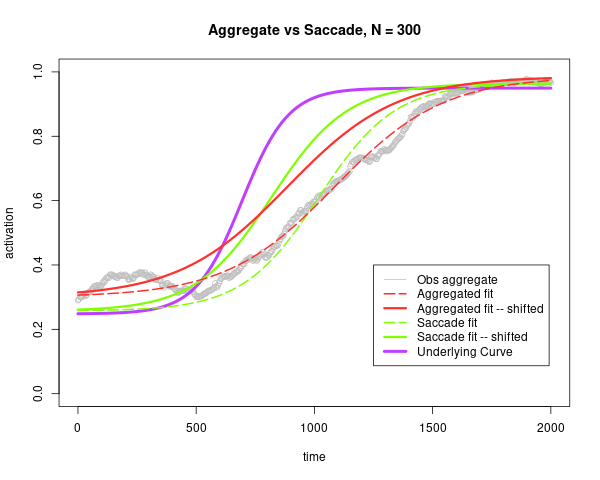
\includegraphics[scale=0.35]{img/reg_fit.png}
\end{center}
% latex table generated in R 4.1.2 by xtable 1.8-4 package
% Thu Apr  7 11:49:44 2022
{\scriptsize
\begin{table}[H]
\captionsetup{font=scriptsize}
\caption*{MISE}
\centering
\begin{tabular}{cccccc}
  \hline
 & Aggregate & Saccade & Aggregate -- Shifted & Saccade -- Shifted & Underlying \\ 
  \hline
 & 57.86 & 58.10 & 20.65 & 10.84 & 0.00 \\ 
   \hline
\end{tabular}
\end{table}
}
\end{frame}

\begin{frame}{early window}
\begin{center}
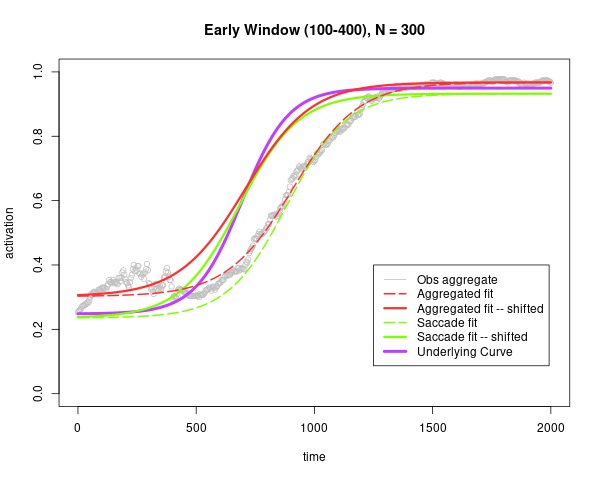
\includegraphics[scale=0.35]{img/early_fit.png}
\end{center}
{\scriptsize
\begin{table}[ht]
\captionsetup{font=scriptsize}
\caption*{MISE}
\centering
\begin{tabular}{cccccc}
  \hline
 & Aggregate & Saccade & Aggregate -- Shifted & Saccade -- Shifted & Underlying \\ 
  \hline
 & 22.51 & 29.94 & 4.18 & 1.14 & 0.00 \\ 
   \hline
\end{tabular}
\end{table}
}
\end{frame}

\begin{frame}{mid window}
\begin{center}
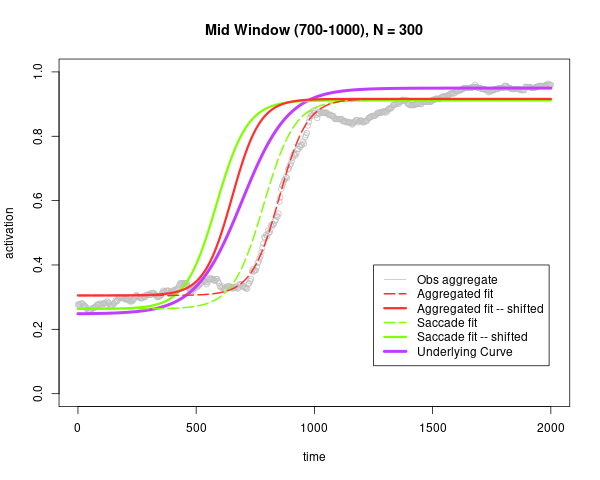
\includegraphics[scale=0.35]{img/mid_fit.png}
\end{center}
{\scriptsize
\begin{table}[ht]
\captionsetup{font=scriptsize}
\caption*{MISE}
\centering
\begin{tabular}{cccccc}
  \hline
 & Aggregate & Saccade & Aggregate -- Shifted & Saccade -- Shifted & Underlying \\ 
  \hline
 & 21.16 & 10.74 & 4.75 & 10.76 & 0.00 \\ 
   \hline
\end{tabular}
\end{table}
}
\end{frame}

\begin{frame}{late window}
\begin{center}
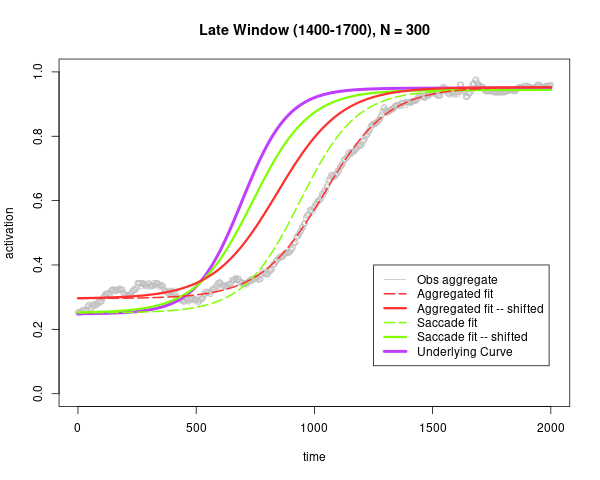
\includegraphics[scale=0.35]{img/late_fit.png}
\end{center}
{\scriptsize
\begin{table}[ht]
\captionsetup{font=scriptsize}
\caption*{MISE}
\centering
\begin{tabular}{cccccc}
  \hline
 & Aggregate & Saccade & Aggregate -- Shifted & Saccade -- Shifted & Underlying \\ 
  \hline
 & 61.89 & 42.18 & 12.77 & 2.18 & 0.00 \\ 
   \hline
\end{tabular}
\end{table}
}
\end{frame}

\begin{frame}{asymptotics}
\begin{center}
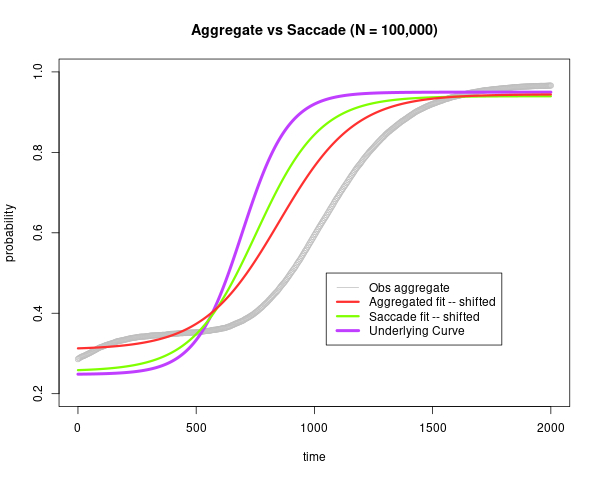
\includegraphics[scale=0.35]{img/asy_fit.png}
\end{center}
{\scriptsize
\begin{table}[ht]
\captionsetup{font=scriptsize}
\caption*{MISE}
\centering
\begin{tabular}{cccc}
 \hline
 & Aggregate -- Shifted & Saccade -- Shifted & Underlying \\ 
  \hline
  & 15.57 & 4.31 & 0.00 \\ 
   \hline
\end{tabular}
\end{table}
}
\end{frame}

\begin{frame}{mise}

It's worth pointing out that each time window will appear better than the trial with no time window, as these ultimately ended up including more samples per trial

{\scriptsize
% latex table generated in R 4.1.2 by xtable 1.8-4 package
% Thu Apr  7 12:22:35 2022
\begin{table}[ht]
\centering
\captionsetup{font=scriptsize}
\caption*{MISE}
\begin{tabular}{cccccc}
  \hline
 & Standard & Early & Mid & Late & N \\ 
  \hline
Aggregate & 57.86 & 22.51 & 21.16 & 61.89 & NA \\ 
  Saccade & 58.10 & 29.94 & 10.74 & 42.18 & NA \\ 
  Aggregate -- Shifted & 20.65 & 4.18 & 4.75 & 12.77 & 15.57 \\ 
  Saccade -- Shifted & 10.84 & 1.14 & 10.76 & 2.18 & 4.31 \\ 
  Underlying & 0.00 & 0.00 & 0.00 & 0.00 & 0.00 \\ 
   \hline
\end{tabular}
\end{table}
}
\end{frame}

\begin{frame}{other issues}
Density of saccades over time \newline \\
identity theorem \newline \\
still does 0-2000ms (how to deal with identifying target/RT) \newline \\
``Ignores the role of the fixation as an information gathering behavior" \newline \\

Can show sims demonstrating time/density/etc with saccades and  wolololo
\end{frame}

\begin{frame}[fragile]
\frametitle{current simulation (fbs+t)}
Begin by creating a subject \newline \\

  \begin{enumerate}
  \item[1.] Draw $\theta \sim N(\theta^*, \Sigma_{\theta^*})$ s.t $max(f_{\theta}) \in (0.6, 1)$
  \item[2.] Draw parameters for distribution $\Gamma$ for duration of fixation to non-target
  \item[3.] Draw parameters for distribution $\Gamma_T$ for duration of fixation to target
  \item[4.] Return $(\theta, \Gamma, \Gamma_T)$
  \end{enumerate}

\end{frame}

\begin{frame}{Current sim (fbs+t)}
Single trial. With vector of times, \code{time}, run the following simulation:\newline \\

\code{pars <- makeSubject()} \\
\code{currTime <- min(time) - runif(1)}$E(\Gamma)$ \\
\code{lastTime <- currTime - }$\Gamma$\code{ - runif(1)}$E(\Gamma)$\newline \\
\code{while(currTime < max(time) \{} \\
\hspace{4mm} \code{p <- f(lasttime|}$\theta$\code{)} \\
\hspace{4mm} \code{target <- runif(1) < p} \\
\hspace{4mm} \code{duration <- ifelse(target, }$\Gamma$\code{, }$\Gamma_T$\code{)} \\
\hspace{4mm} \code{lasttime <- currTime} \\
\hspace{4mm} \code{currTime <- currTime + duration} \\
\code{\}}
\end{frame}

\begin{frame}{Limitations}
Not really recovering cognitive curve \newline 

\end{frame}



\end{document}